\documentclass[12pt]{ctexart}
\usepackage[a4paper,margin=1in]{geometry}
\usepackage{amsmath,amssymb}
\usepackage{xcolor}
\usepackage{graphicx}
\usepackage{tikz}
\usetikzlibrary{positioning,arrows.meta,shapes.geometric}
\usepackage{longtable}
\usepackage{subcaption}
\usepackage{algorithm}
\usepackage{algpseudocode}
\makeatletter
\def\maxwidth{\ifdim\Gin@nat@width>\linewidth\linewidth\else\Gin@nat@width\fi}
\def\maxheight{\ifdim\Gin@nat@height>\textheight\textheight\else\Gin@nat@height\fi}
\makeatother
\setkeys{Gin}{width=\maxwidth,height=\maxheight,keepaspectratio}
\setlength{\emergencystretch}{3em}
\providecommand{\tightlist}{%
  \setlength{\itemsep}{0pt}\setlength{\parskip}{0pt}}
\setcounter{secnumdepth}{-\maxdimen}
\usepackage{bookmark}
\usepackage{xurl}
\urlstyle{same}
\hypersetup{hidelinks,pdfcreator={LaTeX via pandoc}}
\author{}
\date{}

\begin{document}

目 录

1 引言 \hyperref[ux5f15ux8a00]{1}

\hyperref[ux76f8ux5173ux5de5ux4f5c]{2 相关工作
\hyperref[ux76f8ux5173ux5de5ux4f5c]{2}}

\hyperref[ux95eeux9898ux5b9aux4e49]{3 问题定义
\hyperref[ux95eeux9898ux5b9aux4e49]{3}}

\hyperref[ux65b9ux6cd5-proposed-rl-macpo]{4 方法 (Proposed RL-MACPO)
\hyperref[ux65b9ux6cd5-proposed-rl-macpo]{6}}

\hyperref[ux6574ux4f53ux6846ux67b6-ux7b80ux8981ux4ecbux7ecdux4e09ux5927ux6539ux8fdbux673aux5236ux53caux5176ux5173ux7cfb]{4.1
整体框架 (简要介绍三大改进机制及其关系)
\hyperref[ux6574ux4f53ux6846ux67b6-ux7b80ux8981ux4ecbux7ecdux4e09ux5927ux6539ux8fdbux673aux5236ux53caux5176ux5173ux7cfb]{5}}

\hyperref[ux57faux4e8eux5f3aux5316ux5b66ux4e60ux7684ux81eaux9002ux5e94ux60e9ux7f5aux6743ux91cdux8c03ux6574ux673aux5236-ux5982ux4f55ux52a8ux6001ux8c03ux6574ux60e9ux7f5aux5f3aux5ea6]{4.2
基于强化学习的自适应惩罚权重调整机制 (如何动态调整惩罚强度)
\hyperref[ux57faux4e8eux5f3aux5316ux5b66ux4e60ux7684ux81eaux9002ux5e94ux60e9ux7f5aux6743ux91cdux8c03ux6574ux673aux5236-ux5982ux4f55ux52a8ux6001ux8c03ux6574ux60e9ux7f5aux5f3aux5ea6]{6}}

\hyperref[ux57faux4e8eux51b2ux7a81ux6307ux6570ux7684ux95e8ux63a7ux901aux4fe1ux673aux5236-ux51b3ux5b9aux4f55ux65f6ux8fdbux884cux534fux5546]{4.3
基于冲突指数的门控通信机制 (决定何时进行协商)
\hyperref[ux57faux4e8eux51b2ux7a81ux6307ux6570ux7684ux95e8ux63a7ux901aux4fe1ux673aux5236-ux51b3ux5b9aux4f55ux65f6ux8fdbux884cux534fux5546]{12}}

\hyperref[ux667aux80fdux53d8ux91cfux7b5bux9009ux673aux5236-ux51b3ux5b9aux534fux5546ux54eaux4e9bux53d8ux91cf]{4.4
智能变量筛选机制 (决定协商哪些变量)
\hyperref[ux667aux80fdux53d8ux91cfux7b5bux9009ux673aux5236-ux51b3ux5b9aux534fux5546ux54eaux4e9bux53d8ux91cf]{14}}

\hyperref[ux7b80ux5316ux51b2ux7a81ux68c0ux6d4bux4e0eux589eux5f3aux534fux5546ux673aux5236-ux5982ux4f55ux9ad8ux6548ux5730ux8fdbux884cux534fux5546]{4.5
简化冲突检测与增强协商机制 (如何高效地进行协商)
\hyperref[ux7b80ux5316ux51b2ux7a81ux68c0ux6d4bux4e0eux589eux5f3aux534fux5546ux673aux5236-ux5982ux4f55ux9ad8ux6548ux5730ux8fdbux884cux534fux5546]{16}}

\textbf{\hfill\break
}

\subsection{引言}\label{ux5f15ux8a00}

基于网络的分布式优化（Network-based Distributed Optimization,
NDO）旨在解决一种典型的网络系统优化问题：在全局目标不可直接获取的情况下，多个
agent
只能依赖各自有限的局部信息共同优化系统性能。这里的局部信息通常指每个
agent 或计算节点能够访问的局部目标函数，而全局目标只能通过多 agent
的交互与协作间接实现。

在分布式优化中，agent 的决策变量可分为两类：一类是共享变量，由多个 agent
共同控制，例如无线传感器网络中的位置坐标、分布式学习中的模型参数等；另一类是私有变量，仅属于单个
agent，例如电力系统中的节点电压或功率。许多实际问题同时包含共享与私有变量，例如交通网络中的流量优化、电力系统的潮流分布等，这类问题更能体现多
agent 系统的异构性与复杂耦合特征。

现有分布式优化方法大体可分为基于梯度的方法和无梯度的方法。前者依赖于目标函数的可微性，代表性算法包括分布式子梯度下降
(DGD)、交替方向乘子法（ADMM）等；后者则不依赖梯度信息，典型方法如随机无梯度方法
(RGFs)。然而，NDO 的求解面临两类核心技术挑战：一是传统方法依赖凸性、可分解性与梯度可得等假设，难以适应实际系统中高度非线性耦合的复杂场景；二是工程系统中目标函数往往仅能通过仿真或运行反馈评估，呈现典型的黑箱特性，使得基于解析模型的方法失效。与上述方法相比，进化算法 (Evolutionary Computation, EC)
不要求问题具备可微性或凸性，因此更适合处理黑箱与非凸优化问题，尤其是在并行分布式环境下。近年来，强化学习等学习型方法被逐步引入优化领域，用于辅助参数调节与策略选择，为缓解人工经验依赖、提升算法自适应能力提供了新思路。

在这一背景下，我们研究的 NDO
问题首次将共享变量与私有变量同时纳入黑箱和非凸分布式优化的框架。这种设定能够模拟多种现实场景，但也带来了新的挑战：共享变量会引发
agent
之间的冲突，通信和协作开销随网络规模急剧增加。因此，需要设计能够同时兼顾优化质量与计算成本的多
agent 协同演化算法。

然而，现有方法在应对 NDO 时仍存在明显不足。以多 agent
协同演化的代表性方法 MACPO
为例，该算法通过在局部评估中引入惩罚项来处理共享变量冲突，并在邻居间进行逐维协商以保证一致性。虽然这种机制在一定程度上提高了分布式优化的适应性，但它也存在三方面局限：其一，惩罚权重通常是固定设置的，缺乏动态调节能力；其二，协商阶段需要在所有共享变量上进行完整的双向扰动检测，计算开销随维度线性增加；其三，每轮迭代都必须触发通信，导致在大规模问题中通信负担显著。

针对这些问题，本文提出了一种基于强化学习的改进算法（RL-MACPO）。该方法利用强化学习策略动态调整惩罚权重，并结合基于冲突指数的门控通信机制，在 F1--F6 基准上观察到更优的最终适应度；变量筛选作为可插拔扩展机制，在消融实验中表现出对稳定性的边际增益。实验结果表明，RL-MACPO 在多数基准函数上显著优于原始 MACPO。

\subsection{相关工作}\label{ux76f8ux5173ux5de5ux4f5c}

网络型分布式优化（Network-based Distributed Optimization,
NDO）广泛存在于交通分配、电力调度、分布式状态估计等场景中。在 NDO
中，系统由多个 agent 构成，每个 agent
对应网络图中的一个节点，并拥有私有的局部目标函数。其决策变量既包括节点自身的私有变量，也包括连接边上的共享变量。全局目标函数是所有局部目标函数的总和，优化的关键在于：在仅依赖局部信息的条件下，通过相邻
agent
的交互与协作，获得全局最优或次优解。由于共享变量引入了强烈的耦合性，NDO
的求解需要同时处理 agent
间冲突和分布式通信开销，这区别于传统的集中式或并行优化问题。

\textbf{传统分布式优化方法及其局限。}围绕一致性与分解—协调思想，研究者提出了分布式次梯度方法（DGD）、交替方向乘子法（ADMM）等，在凸假设条件下建立了较为完善的收敛性分析框架。然而，这些方法的有效性通常依赖于目标函数与约束的凸性与可分解性、梯度或次梯度信息可得等前提。在实际工程系统中，约束关系往往高度非线性耦合，目标函数仅能通过有限次评估获取反馈，上述假设难以满足，从而限制了传统方法在黑箱与非凸 NDO 场景中的适用范围。

\textbf{黑箱约束优化与惩罚机制。}针对模型不完全可得或难以解析建模的现实需求，黑箱优化逐渐成为重要研究方向。在黑箱约束优化中，惩罚函数法通过将约束违反程度映射为目标函数的一部分，引导优化过程逐步逼近可行区域，被广泛用于复杂约束问题。然而，现有惩罚机制多采用静态规则或人工经验设定，参数依赖性强，难以适应约束冲突程度的动态变化。

\textbf{多智能体协同进化与 MACPO。}为解决上述挑战，Chen
等人提出了基于惩罚目标的多智能体协同进化算法（MACPO）。在该框架中，每个
agent
维护一个子群体，在\textbf{局部优化阶段}利用带惩罚的目标函数演化自身解，在\textbf{协商阶段}通过通信与邻居交换候选解，并在评估、竞争、共享和冲突检测的多步交互中逐步达成共识。惩罚项的设计使得共享变量趋向于共识解，从而增强了全局一致性。MACPO
还通过冲突检测机制自适应调整惩罚开关，在一定程度上缓解了不同子问题之间的目标冲突。

尽管 MACPO 为 NDO
提供了一个有效的解决方案，但仍存在若干局限。首先，惩罚权重在实现中往往采用静态或预设策略，难以根据动态冲突情况灵活调整。其次，协商阶段在所有共享变量上逐维进行完整的扰动和评估，导致计算开销随问题规模线性甚至超线性增加。再次，通信机制在每轮迭代中都会被触发，当网络规模扩大时，通信负担成为主要瓶颈。这些不足限制了
MACPO 在高维、强冲突或大规模网络优化中的效率和扩展性。

\textbf{强化学习赋能优化算法。}在复杂工程系统中，目标函数与约束关系往往难以通过解析模型精确刻画，且系统状态可能随时间变化，使得依赖固定参数或静态规则的优化方法难以长期维持稳定性能。强化学习作为一种基于交互反馈进行策略更新的方法，近年来被广泛用于优化算法中的参数控制、算子选择与决策调节，被视为缓解人工经验依赖、提升算法适应性的重要工具。然而，现有工作多集中于无约束或简单约束问题，对于大规模分布式黑箱优化中惩罚参数与多智能体协同策略的学习机制研究仍较为有限。

针对上述不足，本文提出了一种基于强化学习的改进框架（RL-MACPO）。该方法在延续 MACPO 局部优化与协商机制的基础上，做出两方面核心改进：首先，引入强化学习机制动态调整惩罚权重，使其能够根据冲突程度自适应更新；其次，结合冲突指数（CI）提出门控通信机制，避免在低冲突回合中冗余的信息交换。此外，本文实现了可选的智能变量筛选策略作为扩展机制。这些改进使 RL-MACPO 在 F1--F6 基准上显著优于原始 MACPO。


\subsection{问题定义}\label{ux95eeux9898ux5b9aux4e49}

本文采用 Chen 等人提出的网络型分布式优化（NDO）形式化定义。考虑由 \(n\) 个 agent 构成的网络，用无向图 \(G = (V, E)\) 表示，其中顶点 \(i \in V\) 表示 agent，边 \((i, j) \in E\) 表示 agent 之间的连接。记全局决策变量为 \(X = [x_1, x_2, \ldots, x_D]\)。

对于 agent \(i\)，其局部目标函数由该顶点及其相连边上的变量共同决定。agent \(i\) 的局部变量定义为
\[
X_i = \mathrm{col}\{x_d\}_{d \in \Theta_i}, \quad \Theta_i = I_i \cup \bigcup_{j \in N_i} I_{i,j}
\]
其中 \(I_i \subseteq \{1, 2, \ldots, D\}\) 为顶点 \(i\) 上的\textbf{私有变量}索引集，\(I_{i,j} \subseteq \{1, 2, \ldots, D\}\) 为边 \((i,j)\) 上的\textbf{共享变量}索引集（由 agent \(i\) 与 \(j\) 共同控制），\(N_i := \{j \in V \setminus \{i\} : (i,j) \in E\}\) 为 agent \(i\) 的邻居集合。

NDO 的全局目标函数定义为
\[
\min_{X \in \mathbb{R}^D} \quad F(X) = \sum_{i=1}^{n} f_i(X_i)
\]
其中 \(f_i : \mathbb{R}^{|X_i|} \to \mathbb{R}\) 为 agent \(i\) 的局部目标函数。在分布式设定下，上述问题等价于
\[
\min_{X_1, \ldots, X_n} \sum_{i=1}^{n} f_i(X_i) \quad \text{s.t.} \quad x_i^d = x_j^d,\ \forall d \in I_{i,j},\ \forall (i,j) \in E
\]
其中边 \((i,j)\) 上的共享变量 \(x^d\) 在 agent \(i\) 与 \(j\) 处分别记为 \(x_i^d\) 与 \(x_j^d\)，约束要求相邻 agent 在共享变量上达成一致。由于私有变量与共享变量在局部目标中耦合，且网络具有传递性，所有 agent 需通过通信与协作共同求解该优化问题。本文在相同问题设定下，针对 MACPO 的若干局限提出改进。

\subsection{MACPO 原框架回顾}\label{sec:macpo_prelim}

为便于界定本文改进点，本节先回顾原始 MACPO 的标准求解框架。MACPO 面向 NDO 的核心思想是：在每个 agent 的局部演化过程中引入冲突惩罚项，并通过邻居协商逐步压缩共享变量分歧，从而在“局部优化能力”与“跨节点一致性”之间取得平衡。

对 agent \(i\) 而言，原框架在局部阶段优化惩罚目标
\[
h_i(x)=f_i(x)+\alpha_i\,c_i(x),
\]
其中 \(f_i(x)\) 为局部目标，\(c_i(x)\) 刻画与邻域共识解的偏差，\(\alpha_i\) 为惩罚权重。该设计使每个 agent 在保持局部搜索能力的同时，对共享变量一致性施加约束。

基于该目标，MACPO 的一轮迭代可概括为两个主阶段：
\begin{itemize}
\item \textbf{局部优化阶段（Local Optimization）}：每个 agent 独立维护并演化本地种群，得到局部最优候选解；
\item \textbf{邻居协商阶段（Neighbor Negotiation）}：相邻 agent 交换候选解后，在共享维度上执行评估、竞争与写回，以更新共识参考并减小冲突。
\end{itemize}

在协商细节上，原框架通常采用“逐维比较 + 冲突检测”的流程：先依据双方效用对共享变量逐维决策，再通过扰动响应判断是否继续在该维度协商。该机制能够在黑箱条件下实现可行的一致性推进，是 MACPO 相较于传统集中式方法的重要优势。

然而，原始 MACPO 也存在三类已知瓶颈：其一，惩罚权重多依赖静态或经验设定，难以随冲突动态自适应；其二，协商阶段往往在较多共享维度上进行完整评估，计算开销较高；其三，通信触发较为频繁，在大规模网络中易形成额外负担。本文提出的 RL-MACPO 正是在保持上述“局部优化 + 协商”主框架不变的前提下，对权重更新、通信触发与协商执行策略进行系统改进。

\subsection{方法 (Proposed
RL-MACPO)}\label{ux65b9ux6cd5-proposed-rl-macpo}

为克服这些不足，我们提出了改进的 RL-MACPO 框架。在继承 MACPO 基础流程的同时，RL-MACPO 引入了两项核心机制与一项扩展机制。核心机制之一是强化学习自适应惩罚权重，通过策略网络动态更新惩罚系数，使算法能够随冲突状态变化而灵活调整局部目标与一致性约束之间的平衡；另一项核心机制是基于相对冲突水平的门控通信，通过相对 CI 阈值、阶段采样与保底触发联合决定是否进入协商分支，从而避免固定绝对阈值带来的 zero-comm 退化。除此之外，本文还实现了智能变量筛选与协商开关控制，作为可插拔扩展模块，用于在协商阶段优先处理更重要的共享维度并减少无效评估。

通过上述改进，RL-MACPO 在保持 MACPO “局部优化 + 邻居协商”主框架可解释性的同时，使惩罚更新更具自适应性，使通信触发更贴合不同函数与不同阶段的冲突尺度，并在实验中表现出更优的最终适应度与更稳健的收敛特性。

\subsection{整体框架
(简要介绍三大改进机制及其关系)}\label{ux6574ux4f53ux6846ux67b6-ux7b80ux8981ux4ecbux7ecdux4e09ux5927ux6539ux8fdbux673aux5236ux53caux5176ux5173ux7cfb}

本文提出的 RL-MACPO 算法继承了 MACPO 的整体框架，即在
\textbf{局部优化阶段}与\textbf{协商阶段}之间交替运行。局部优化阶段主要通过带惩罚项的目标函数引导群体在局部子问题上进行搜索，从而提高个体适应度并维持对全局约束的遵循。协商阶段则由相邻
agent 在共享变量维度上进行信息交互，以实现跨 agent 的一致性控制。

在 MACPO
的原始设计中，协商阶段由三个基本步骤构成，即\textbf{评估（Evaluation）------竞争（Competition）------共享（Sharing）}。在评估环节中，每个
agent 将自身最优解发送给相邻
agent，并计算在共享变量替换下的局部适应度表现；在竞争环节中，两个 agent
基于适应度比较逐维决定共享变量的取值；在共享环节中，竞争结果被写回局部解与全局缓存，从而保证相邻
agent
在共享变量上的一致性。上述流程构成了一个迭代逼近的过程，使得私有变量和共享变量逐步协调，并最终收敛到全局可行解。

尽管该框架在多个分布式优化问题上表现出良好的适应性，但在高维和冲突密集场景下仍存在局限性。其一，原始协商机制在所有共享维度上进行全面评估，导致计算成本随问题规模显著增加；其二，竞争过程仅依赖于即时适应度比较，缺乏对历史信息的利用，因而容易在局部最优附近停滞；其三，冲突检测依赖双侧扰动进行数值梯度估计，计算负担较重且数值稳定性不足。

为克服这些不足，本文在保持原有``局部优化---协商''双阶段的前提下，对协商相关机制进行了系统性改进。新的 RL-MACPO 框架在局部优化阶段引入基于强化学习的惩罚更新，在协商触发阶段引入基于相对冲突水平的门控通信，并保留智能变量筛选与开关控制作为可插拔扩展模块。这样的设计保持了原框架的可解释性，同时把改动集中在最影响冗余开销与收敛稳定性的环节上。这些改进将在下文中分别展开说明。

算法的整体流程如图~\ref{fig:rl_macpo_architecture}(a) 所示，基于强化学习的自适应惩罚更新回路如图~\ref{fig:rl_macpo_architecture}(b) 所示。

% --- Begin RL-MACPO Two-Panel TikZ Figure ---
\begin{figure*}[htbp]
\centering

\begin{subfigure}[t]{0.63\textwidth}
\centering
\resizebox{\linewidth}{!}{%
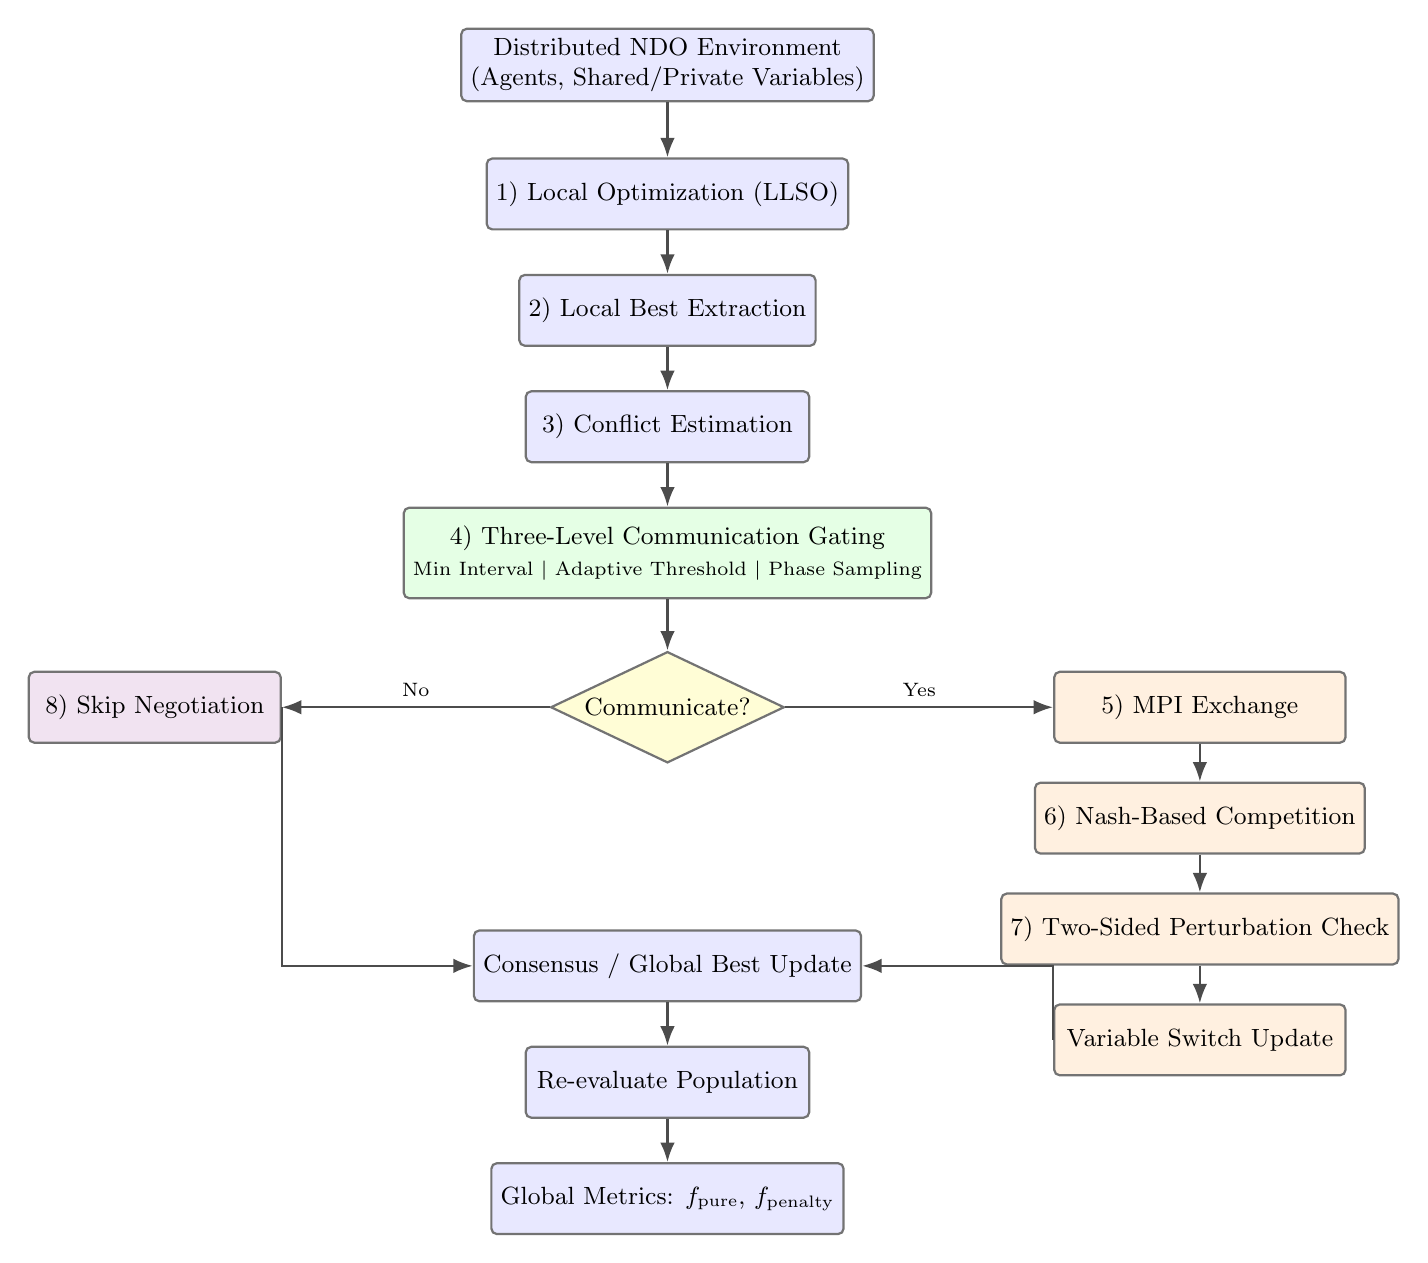
\begin{tikzpicture}[
  font=\small,
  line/.style={-Latex, line width=0.9pt, draw=black!70},
  box/.style={rounded corners=2pt, draw=black!55, line width=0.8pt, minimum width=3.6cm, minimum height=0.90cm, align=center},
  flow/.style={box, fill=blue!9},
  gate/.style={box, fill=green!10, minimum width=4.1cm, minimum height=1.15cm},
  nego/.style={box, fill=orange!12, minimum width=3.7cm},
  skip/.style={box, fill=violet!11, minimum width=3.2cm},
  decision/.style={diamond, draw=black!55, fill=yellow!16, line width=0.8pt, aspect=2.1, inner sep=1.8pt, align=center}
]
% Main pipeline only
\node[flow] (env) at (0,5.7) {Distributed NDO Environment\\(Agents, Shared/Private Variables)};
\node[flow, below=0.70cm of env] (opt) {1) Local Optimization (LLSO)};
\node[flow, below=0.55cm of opt] (best) {2) Local Best Extraction};
\node[flow, below=0.55cm of best] (conf) {3) Conflict Estimation};
\node[gate, below=0.55cm of conf] (gating) {4) Three-Level Communication Gating\\{\scriptsize Min Interval $\mid$ Adaptive Threshold $\mid$ Phase Sampling}};
\node[decision, below=0.65cm of gating] (decide) {Communicate?};

% Branches
\node[nego, right=3.4cm of decide] (ex) {5) MPI Exchange};
\node[nego, below=0.48cm of ex] (nash) {6) Nash-Based Competition};
\node[nego, below=0.48cm of nash] (pert) {7) Two-Sided Perturbation Check};
\node[nego, below=0.48cm of pert] (vsw) {Variable Switch Update};
\node[skip, left=3.4cm of decide] (skp) {8) Skip Negotiation};

% Merge and downstream
\node[flow, below=2.10cm of decide] (cons) {Consensus / Global Best Update};
\node[flow, below=0.55cm of cons] (reeval) {Re-evaluate Population};
\node[flow, below=0.55cm of reeval] (metrics) {Global Metrics: $f_{\mathrm{pure}}$, $f_{\mathrm{penalty}}$};

% Main arrows
\draw[line] (env) -- (opt);
\draw[line] (opt) -- (best);
\draw[line] (best) -- (conf);
\draw[line] (conf) -- (gating);
\draw[line] (gating) -- (decide);

\draw[line] (decide.east) -- node[above, font=\scriptsize] {Yes} (ex.west);
\draw[line] (ex) -- (nash);
\draw[line] (nash) -- (pert);
\draw[line] (pert) -- (vsw);
\draw[line] (vsw.west) |- (cons.east);

\draw[line] (decide.west) -- node[above, font=\scriptsize] {No} (skp.east);
\draw[line] (skp.east) |- (cons.west);

\draw[line] (cons) -- (reeval);
\draw[line] (reeval) -- (metrics);
\end{tikzpicture}%
}
\caption{Main optimization pipeline and communication gating.}
\label{fig:rl_macpo_main}
\end{subfigure}
\hfill
\begin{subfigure}[t]{0.33\textwidth}
\centering
\includegraphics[width=\linewidth]{media/media/RL Adaptive Penalty Loop.png}
\caption{RL-based adaptive penalty update loop.}
\label{fig:rl_macpo_rl}
\end{subfigure}

\caption{Overall Architecture of RL-MACPO. Subfigure (a) shows the main optimization and negotiation pipeline; subfigure (b) shows the RL-based adaptive penalty loop.}
\label{fig:rl_macpo_architecture}
\end{figure*}

\subsection{基于强化学习的自适应惩罚权重调整机制
(如何动态调整惩罚强度)}\label{ux57faux4e8eux5f3aux5316ux5b66ux4e60ux7684ux81eaux9002ux5e94ux60e9ux7f5aux6743ux91cdux8c03ux6574ux673aux5236-ux5982ux4f55ux52a8ux6001ux8c03ux6574ux60e9ux7f5aux5f3aux5ea6}

图~\ref{fig:rl_penalty_loop_png} 展示了 RL 自适应惩罚回路的流程示意，包括状态输入、策略网络、动作输出、比例/权重更新与奖励反馈闭环。

\begin{figure}[htbp]
\centering
\includegraphics[width=0.9\linewidth]{media/media/image1.png}
\caption{RL-Based Adaptive Penalty Loop (Abstract, Code-Aligned)}
\label{fig:rl_penalty_loop_png}
\end{figure}

为与当前实现一致，RL-MACPO 在每个智能体上采用“\textbf{惩罚基准 + 比例调节}”的两层权重机制。局部优化目标写为
\[
h_i(x)=f_i(x)+\alpha_i\,c_i(x),
\]
其中 \(f_i(x)\) 为局部目标，\(c_i(x)\) 为与共识参考解相关的冲突项，\(\alpha_i\) 为自适应惩罚系数。

当前实现中，冲突项采用重叠维度上的归一化距离求和（而非平均）：
\[
c_i(x)=\sum_{d\in\Theta_i}\frac{|x^d-x_{i,\mathrm{con}}^d|}{u_d-l_d}.
\]
该定义保留了冲突规模信息，后续通过 \(\alpha_i\) 的自适应更新进行尺度补偿。

在策略层，每个智能体维护轻量级策略网络 \(\pi_\theta\)，输入状态为
\[
s_i^t=[\,c_i^t,\ \Delta c_i^t\,],\qquad
\Delta c_i^t=c_i^t-c_i^{t-1},
\]
并输出动作
\[
a_i^t=\pi_\theta(s_i^t),\qquad a_i^t\in(-1,1).
\]

与代码一致，惩罚系数不直接回归，而是先更新比例变量再映射到 \(\alpha_i\)：
\[
\rho_i^{t+1}=\Pi_{[\rho_{\min},\rho_{\max}]}\!\left(\rho_i^t+\eta_a a_i^t\right),
\]
\[
\alpha_i^{t+1}=\bar{\alpha}_i^{t+1}\,\rho_i^{t+1}.
\]
其中 \(\Pi\) 表示区间投影算子，\(\bar{\alpha}_i\) 是与目标值量级相关的基准惩罚，\(\rho_i\) 负责在线自适应调节。

奖励信号采用“冲突变化率--纯目标变化率”耦合形式，并经有界非线性映射：
\[
r_i^t=\psi\!\left(-\,\Delta c_{i,\mathrm{rate}}^t\cdot \Delta f_{i,\mathrm{pure,rate}}^t\right),
\]
其中 \(\psi(\cdot)\) 为奇函数有界映射（实现中为 \(\tanh\) 族），用于保证训练稳定并保持奖励符号可解释性。该定义与旧版对数奖励不同，更强调“冲突缓解与目标改进是否同步发生”。

策略学习采用在线更新与经验回放结合：经验三元组 \((s_i^t,a_i^t,r_i^t)\) 写入缓存，按优先级抽样进行小批量更新。优先级由奖励幅度构造：
\[
p_i^t=\phi\!\left(|r_i^t|\right),
\]
其中 \(\phi(\cdot)\) 为单调映射。该机制使高信息量回合在训练中获得更高权重。

\textbf{伪代码一致性说明：} 本文“算法流程图/伪代码图”按机制级抽象给出，不绑定具体常数；其控制流与实现一致，即“状态构建 \(\rightarrow\) 策略前向 \(\rightarrow\) 比例更新 \(\rightarrow\) 惩罚映射 \(\rightarrow\) 奖励反馈 \(\rightarrow\) 经验回放更新”。

\begin{algorithm}[htbp]
\caption{RL-Based Adaptive Penalty Update (Abstract)}
\label{alg:rl_penalty_update}
\begin{algorithmic}[1]
\Require Agent state history, baseline-penalty stream \(\bar{\alpha}_i^t\), replay buffer \(\mathcal{B}_i\), policy \(\pi_{\theta_i}\)
\Ensure Per-iteration updates \(\{\rho_i^t,\alpha_i^t,\theta_i\}\)
\State Initialize \(\rho_i^0\), previous conflict \(c_i^{-1}\), and empty \(\mathcal{B}_i\)
\For{each optimization iteration \(t\)}
  \State Evaluate local conflict \(c_i^t\) from shared-variable discrepancy
  \State Compute trend feature \(\Delta c_i^t \gets c_i^t-c_i^{t-1}\)
  \State Build state \(s_i^t \gets [c_i^t,\Delta c_i^t]\)
  \State Policy inference \(a_i^t \gets \pi_{\theta_i}(s_i^t)\), with \(a_i^t\in(-1,1)\)
  \State Ratio update \(\rho_i^{t+1}\gets \Pi_{[\rho_{\min},\rho_{\max}]}\!\left(\rho_i^t+\eta_a a_i^t\right)\)
  \State Penalty mapping \(\alpha_i^{t+1}\gets \bar{\alpha}_i^{t+1}\rho_i^{t+1}\)
  \State Run local optimization using \(h_i(x)=f_i(x)+\alpha_i^{t+1}c_i(x)\)
  \State Measure pure-objective change rate \(\Delta f_{i,\mathrm{pure,rate}}^t\)
  \State Measure conflict change rate \(\Delta c_{i,\mathrm{rate}}^t\)
  \State Coupled reward \(r_i^t\gets \psi\!\left(-\Delta c_{i,\mathrm{rate}}^t\cdot \Delta f_{i,\mathrm{pure,rate}}^t\right)\)
  \State Push transition \((s_i^t,a_i^t,r_i^t)\) into \(\mathcal{B}_i\)
  \If{replay condition is satisfied}
    \State Compute priority \(p_k\propto \phi(|r_k|)\) for buffered samples
    \State Sample mini-batch by priority and update \(\theta_i\) with policy loss
  \EndIf
  \State Update history state: \(c_i^{t-1}\gets c_i^t\)
\EndFor
\State \Return Updated \(\rho_i,\alpha_i,\theta_i\)
\end{algorithmic}
\end{algorithm}

\subsection{基于冲突指数的门控通信机制
(决定何时进行协商)}\label{ux57faux4e8eux51b2ux7a81ux6307ux6570ux7684ux95e8ux63a7ux901aux4fe1ux673aux5236-ux51b3ux5b9aux4f55ux65f6ux8fdbux884cux534fux5546}

在当前实现中，通信触发采用三层门控，而非“每轮必通信”。与早期固定绝对阈值不同，当前版本使用基于 CI 历史尺度的相对阈值，并在必要时加入保底触发，以避免协商被永久关闭。设 \(g_i^t\in\{0,1\}\) 表示智能体 \(i\) 在第 \(t\) 轮的本地通信建议，则
\[
g_i^t=\mathbf{1}\!\left[\mathcal{C}_{\mathrm{int}}^t\land \mathcal{C}_{\mathrm{thr}}^t\land \mathcal{C}_{\mathrm{phase}}^t\right],
\]
三项条件分别为：
\begin{align}
\mathcal{C}_{\mathrm{int}}^t &: \text{满足最小通信间隔约束},\\
\mathcal{C}_{\mathrm{thr}}^t &: \mathrm{CI}_i^t > \lambda\,\hat{\mu}_{\mathrm{CI},i}^t\ \text{或}\ t-t_{\mathrm{last\_comm}}\ge K,\\
\mathcal{C}_{\mathrm{phase}}^t &: u_i^t < p_{\mathrm{phase}}^t,\quad u_i^t\sim\mathcal{U}(0,1).
\end{align}

其中 \(\mathrm{CI}_i^t\) 由局部解与参考解的鲁棒差异度量得到，\(\hat{\mu}_{\mathrm{CI},i}^t\) 用于刻画当前阶段的 CI 典型尺度，\(\lambda\) 与 \(K\) 分别控制相对阈值强度和最长静默轮次，\(p_{\mathrm{phase}}^t\) 则进一步调节不同阶段的通信频率。相比固定绝对阈值，该门控更符合 CI 随函数和优化阶段变化的事实，也更不容易出现零触发退化。

在并行实现中，系统通过全局归并得到最终通信决策：
\[
g_{\mathrm{global}}^t=\max_i g_i^t.
\]
当任一智能体触发通信时，相关邻域进入协商分支；否则直接沿“跳过协商”分支更新共识参考。

\textbf{伪代码一致性说明：} 门控伪代码应包含“间隔约束 + 阈值判定 + 阶段采样 + 全局归并”四个环节；若缺失其中任一环节，则与当前实现不一致。

\begin{algorithm}[htbp]
\caption{CI-Gated Communication with Phase Sampling (Abstract)}
\label{alg:ci_gating}
\begin{algorithmic}[1]
\Require Local-best \(x_i^\star\), consensus reference \(x_{i,\mathrm{con}}\), overlap set \(\Theta_i\), communication records
\Ensure Global gate \(g_{\mathrm{global}}^t\), communication branch selection
\For{each optimization iteration \(t\)}
\State Compute local conflict index \(\mathrm{CI}_i^t\) on \(\Theta_i\)
\State Update EMA statistic \(\hat{\mu}_{\mathrm{CI},i}^t\) and the last-communication record
\State Check interval constraint \(\mathcal{C}_{\mathrm{int}}^t\) from communication cooldown
\State Check threshold constraint
\[
\mathcal{C}_{\mathrm{thr}}^t : \mathrm{CI}_i^t > \lambda\hat{\mu}_{\mathrm{CI},i}^t\ \text{or}\ t-t_{\mathrm{last\_comm}}\ge K
\]
  \State Draw phase sample \(u_i^t\sim\mathcal{U}(0,1)\) and check \(\mathcal{C}_{\mathrm{phase}}^t : u_i^t<p_{\mathrm{phase}}^t\)
  \State Local gate
  \[
  g_i^t\gets \mathbf{1}\!\left[\mathcal{C}_{\mathrm{int}}^t\land \mathcal{C}_{\mathrm{thr}}^t\land \mathcal{C}_{\mathrm{phase}}^t\right]
  \]
  \State Global reduction \(g_{\mathrm{global}}^t\gets \max_i g_i^t\)
  \If{\(g_{\mathrm{global}}^t=0\)}
    \State Follow skip-negotiation branch and keep local evolution only
    \State Refresh consensus reference from local-best maintenance rule
  \Else
    \State Enter negotiation branch for active neighbor pairs
    \State Execute exchange \(\rightarrow\) competition \(\rightarrow\) consistency check \(\rightarrow\) sharing
  \EndIf
  \State Update communication counters, interval timers, and threshold state
\EndFor
\State \Return Communication decisions and branch traces
\end{algorithmic}
\end{algorithm}

为验证门控规则的必要性，本文额外设计了一个最小机制实验，在 F1、F2、F5 三个代表性函数上比较四种通信策略：Always-on（V0）、固定绝对阈值（V1）、相对阈值（V2）以及相对阈值加保底触发（V3）。结果表明，固定绝对阈值会将通信完全锁死，而相对阈值与保底触发能够恢复“稀疏但非零”的协商过程。

进一步地，从 30 次运行的聚合统计看，V1 的通信触发率为 0，且 \(30/30\) 次运行均出现 zero-comm；V2 与 V3 的平均通信触发率分别为 \(0.504\pm0.055\) 与 \(0.460\pm0.069\)，通信轮次相对 Always-on 分别下降 \(49.58\%\) 与 \(54.03\%\)，且均未出现 zero-comm 运行。该结果说明，相对阈值并非单纯增加通信，而是在保持非零协商能力的前提下显著压缩冗余交互。

\subsection{智能变量筛选机制
(决定协商哪些变量)}\label{ux667aux80fdux53d8ux91cfux7b5bux9009ux673aux5236-ux51b3ux5b9aux534fux5546ux54eaux4e9bux53d8ux91cf}

图~\ref{fig:smart_selection_png} 给出了智能变量筛选与开关控制流程示意，体现“重要性估计--候选判定--一致性检测--开关更新”的执行链路。

\begin{figure}[htbp]
\centering
\includegraphics[width=0.9\linewidth]{media/media/image2.png}
\caption{Smart Variable Selection and Switch Control (Abstract, Code-Aligned)}
\label{fig:smart_selection_png}
\end{figure}

智能变量筛选的目标是在协商阶段优先处理高影响维度。对每个共享变量 \(d\) 定义重要性分数 \(q_d^t\)，其更新可写为
\[
q_d^{t+1}=\gamma q_d^t+(1-\gamma)\,\xi_d^t,
\]
其中 \(\xi_d^t\) 由冲突贡献与历史协商成效共同构成，\(\gamma\in(0,1)\) 为平滑系数。

在候选维度集合 \(\Theta_i\) 上，按 \(q_d^t\) 排序并选择子集 \(\Omega_i^t\subseteq\Theta_i\) 参与协商，随后在 \(\Omega_i^t\) 上执行逐维试探与一致性判定。该机制本质上是“\textbf{先筛选、再协商}”，用于降低维度级协商开销。

\textbf{与当前主程序的一致性说明：}
\begin{itemize}
\item 该模块在评估器中已具备完整接口与状态维护逻辑；
\item 当前默认主流程中，显式 Top-\(R\) 维度筛选未作为硬前置步骤启用；
\item 默认流程仍通过门控通信与维度开关（\(\mathrm{variable\_switch}\)）抑制无效协商。
\end{itemize}

因此，本文将该机制定位为“可插拔扩展模块”：其思想与接口与实现一致，但是否在主实验配置中启用由实验设置决定。

\subsection{简化冲突检测与增强协商机制
(如何高效地进行协商)}\label{ux7b80ux5316ux51b2ux7a81ux68c0ux6d4bux4e0eux589eux5f3aux534fux5546ux673aux5236-ux5982ux4f55ux9ad8ux6548ux5730ux8fdbux884cux534fux5546}

当前实现中的协商分支由“解交换、竞争判定、扰动一致性检测、共享写回”组成，控制流与主程序一致。

\textbf{(1) 竞争判定（Nash-style）}  
对每个共享维度 \(d\)，构造双方在本地/交叉评估下的效用量并进行比较。若
\[
u_{\mathrm{self}}(d)+u_{\mathrm{cross}\rightarrow\mathrm{self}}(d)
>
u_{\mathrm{cross}}(d)+u_{\mathrm{self}\rightarrow\mathrm{cross}}(d),
\]
则采用邻居值；否则保持本地值。该判据等价于在共享维度上进行双边增益比较。

\textbf{(2) 双侧扰动一致性检测}  
竞争后对候选维度执行正向/负向双侧扰动检测。记双方在维度 \(d\) 上的扰动响应为
\((\delta_i^+,\delta_i^-)\) 与 \((\delta_j^+,\delta_j^-)\)，若
\[
(\delta_i^+\delta_j^+>0)\land(\delta_i^-\delta_j^->0),
\]
则认为两侧方向一致，该维度关闭协商开关；否则保留竞争结果并允许共享写回。该规则与代码中的 \(\mathrm{variable\_switch}\) 更新逻辑一致。

\textbf{(3) 共享写回与重评估}  
通过检测的维度写入共识参考解，随后对种群进行重评估并进入下一轮迭代。未通过维度保持局部值，避免无效更新。

\textbf{复杂度与鲁棒性含义：}
\begin{itemize}
\item 协商只在“门控通信触发 + 维度开关保留”的条件下执行，显著降低冗余开销；
\item 双侧扰动检测以符号一致性为核心，避免了对复杂高阶信息的依赖；
\item 与前述门控机制结合后，协商分支可在保持一致性的同时提高并行效率。
\end{itemize}

\textbf{伪代码一致性说明：} 当前伪代码应体现“先竞争、后双侧扰动检测、再按 \(\mathrm{variable\_switch}\) 写回”的顺序；若写成单侧扰动或省略开关更新，则与实现不一致。

\begin{algorithm}[htbp]
\caption{Negotiation with Two-Sided Consistency Check (Abstract)}
\label{alg:negotiation_consistency}
\begin{algorithmic}[1]
\Require Neighbor pair \((i,j)\), local-best candidates \(x_i^\star,x_j^\star\), shared set \(L_{i,j}\), variable switch \(\mathrm{switch}[\cdot]\)
\Ensure Updated shared variables, consensus reference, and negotiation-success flag
\State Exchange \(x_i^\star\) and \(x_j^\star\) between neighbors
\State Initialize negotiation-success flag as false
\For{each shared dimension \(d\in L_{i,j}\)}
  \If{\(\mathrm{switch}[d]=0\)}
    \State \textbf{continue} \Comment{dimension already closed}
  \EndIf
  \State Build local trial and cross trial for dimension \(d\)
  \State Evaluate utilities \(u_{\mathrm{self}}(d),u_{\mathrm{cross}}(d),u_{\mathrm{cross}\rightarrow\mathrm{self}}(d),u_{\mathrm{self}\rightarrow\mathrm{cross}}(d)\)
  \If{\(u_{\mathrm{self}}(d)+u_{\mathrm{cross}\rightarrow\mathrm{self}}(d) > u_{\mathrm{cross}}(d)+u_{\mathrm{self}\rightarrow\mathrm{cross}}(d)\)}
    \State Select neighbor value for \(d\)
  \Else
    \State Keep local value for \(d\)
  \EndIf
  \State Perform two-sided perturbation around selected value on \(d\)
  \State Obtain responses \((\delta_i^+,\delta_i^-)\) and \((\delta_j^+,\delta_j^-)\)
  \If{\((\delta_i^+\delta_j^+>0)\land(\delta_i^-\delta_j^->0)\)}
    \State \(\mathrm{switch}[d]\gets 0\) \Comment{consistent direction, stop negotiating \(d\)}
  \Else
    \State Keep \(\mathrm{switch}[d]\) active and allow future renegotiation
  \EndIf
  \State If accepted by sharing rule, write updated \(d\) into consensus reference
  \State Update negotiation-success flag when at least one shared dimension is effectively changed
\EndFor
\State Re-evaluate local population under new consensus reference
\State \Return Consensus reference, \(\mathrm{switch}[\cdot]\), negotiation-success flag
\end{algorithmic}
\end{algorithm}

\subsection{实验设置与结果}\label{sec:experiments}

\subsection{实验设置}


\subsection{主对比结果}

表~\ref{tab:main} 汇总了原始 MACPO、仅 RL（RL\_Only\_SimpleRL）、完整系统（Full\_LLSO）以及外部基线（DPSO、GFPDO）在 6 个基准函数上的适应度均值与改善率。其中 Full 配置包含 RL 自适应惩罚、CI 门控通信与 variable\_switch 机制；显式 Top-k 变量筛选在消融实验中单独评估，主表结果不依赖其硬启用。

\begin{table}[htbp]
\centering
\caption{Results on LLSO Benchmark (25 Runs)}
\label{tab:main}
\resizebox{\textwidth}{!}{%
\begin{tabular}{lcccccc}
\hline
方法 & F1 & F2 & F3 & F4 & F5 & F6 \\
\hline
原始 MACPO & 1.98E7 & 5.05E4 & 4.03E9 & 3.17E6 & 1.97E8 & 1.62E8 \\
RL\_Only & 2.07E7 (-5\%) & 4.76E4 (6\%) & 5.89E9 (-46\%) & 3.01E6 (5\%) & 4.24E8 (-115\%) & 1.50E8 (7\%) \\
Full & 6.36E6 (68\%) & 3.29E3 (93\%) & 6.40E2 (100\%) & 2.59E6 (18\%) & 3.44E6 (98\%) & 2.50E3 (100\%) \\
DPSO & 2.25E10 (-113734\%) & 5.61E10 (-111087028\%) & 3.86E10 (-858\%) & 1.68E10 (-529649\%) & 2.65E10 (-13373\%) & 2.72E10 (-16695\%) \\
GFPDO & 8.46E8 (-4173\%) & 9.26E6 (-18247\%) & 5.86E10 (-1354\%) & 4.53E8 (-14190\%) & 2.11E10 (-10604\%) & 4.00E10 (-24540\%) \\
\hline
\end{tabular}%
}
\end{table}

表~\ref{tab:main_cso} 汇总了原始 MACPO、RL\_Only、完整系统以及外部基线在 CSO 基准测试集上的适应度均值与改善率（25 次运行）。

\begin{table}[htbp]
\centering
\caption{Results on CSO Benchmark (25 Runs)}
\label{tab:main_cso}
\resizebox{\textwidth}{!}{%
\begin{tabular}{lcccccc}
\hline
方法 & F1 & F2 & F3 & F4 & F5 & F6 \\
\hline
原始 MACPO & 2.33E7 & 6.95E4 & 1.51E9 & 7.30E6 & 2.50E7 & 3.40E6 \\
RL\_Only & 2.02E7 (13\%) & 6.43E4 (8\%) & 2.66E9 (-76\%) & 6.98E6 (4\%) & 4.98E7 (-99\%) & 4.29E5 (87\%) \\
Full & 1.25E7 (46\%) & 9.11E3 (87\%) & 6.70E2 (100\%) & 5.80E6 (20\%) & 6.61E6 (74\%) & 5.56E3 (100\%) \\
DPSO & 3.65E10 (-156330\%) & 2.69E10 (-38704812\%) & 3.99E10 (-2542\%) & 1.89E10 (-258804\%) & 4.30E10 (-171823\%) & 4.00E10 (-1176403\%) \\
GFPDO & 2.06E10 (-88226\%) & 2.37E9 (-3409956\%) & 1.04E11 (-6779\%) & 8.62E9 (-118047\%) & 5.60E10 (-223630\%) & 5.23E10 (-1538127\%) \\
\hline
\end{tabular}%
}
\end{table}

表~\ref{tab:macpo_style} 按 MACPO 原论文 Table I 格式，进一步给出 mean、median、std 及 Wilcoxon 秩和检验的 p-value（$\alpha=0.05$），其中 * 表示显著优于 MACPO，\# 表示显著劣于 MACPO；w/t/l 为各方法相对 MACPO 的胜/平/负次数。

{\small
\setlength{\LTleft}{0pt}
\setlength{\LTright}{0pt}
\begin{longtable}{lccccc}
\caption{Comparison with MACPO (25 Runs, LLSO). Mean, median, std in separate rows. * significantly better than MACPO; \# significantly worse (Wilcoxon, $\alpha=0.05$). All methods are measured under the same implementation and evaluation-budget settings.}
\label{tab:macpo_style}\\
\hline
\textbf{Function} & \textbf{MACPO} & \textbf{RL Only} & \textbf{RL-MACPO} & \textbf{DPSO} & \textbf{GFPDO} \\
\hline
\endfirsthead

\multicolumn{6}{l}{\tablename\ \thetable\ （续）}\\
\hline
\textbf{Function} & \textbf{MACPO} & \textbf{RL Only} & \textbf{RL-MACPO} & \textbf{DPSO} & \textbf{GFPDO} \\
\hline
\endhead

\hline
\multicolumn{6}{r}{续下页}\\
\endfoot

\hline
\endlastfoot

\multicolumn{6}{l}{\textit{F1}} \\
mean & 1.98E+7 & 2.07E+7 & 6.36E+6 & 2.25E+10 & 8.46E+8 \\
median & 2.00E+7 & 1.97E+7 & 6.31E+6 & 2.23E+10 & 8.29E+8 \\
std & 1.67E+6 & 3.58E+6 & 4.25E+5 & 2.66E+9 & 8.46E+7 \\
p-value & - & 5.46e-01 & 7.03e-10* & 9.13e-05\# & 5.46e-06\# \\
\hline
\multicolumn{6}{l}{\textit{F2}} \\
mean & 5.05E+4 & 4.76E+4 & 3.29E+3 & 5.61E+10 & 9.43E+6 \\
median & 4.83E+4 & 4.35E+4 & 3.30E+3 & 1.34E+10 & 9.26E+6 \\
std & 6.10E+3 & 9.67E+3 & 8.82E+2 & 9.39E+10 & 4.13E+6 \\
p-value & - & 2.99e-02* & 7.07e-10* & 9.13e-05\# & 5.46e-06\# \\
\hline
\multicolumn{6}{l}{\textit{F3}} \\
mean & 4.03E+9 & 5.89E+9 & 6.40E+2 & 3.86E+10 & 5.86E+10 \\
median & 4.05E+9 & 5.86E+9 & 6.58E+2 & 3.87E+10 & 5.83E+10 \\
std & 4.69E+8 & 7.13E+8 & 1.92E+2 & 5.62E+8 & 4.22E+9 \\
p-value & - & 1.00e+00\# & 7.07e-10* & 9.13e-05\# & 5.46e-06\# \\
\hline
\multicolumn{6}{l}{\textit{F4}} \\
mean & 3.17E+6 & 3.01E+6 & 2.59E+6 & 1.68E+10 & 4.53E+8 \\
median & 3.14E+6 & 2.98E+6 & 2.56E+6 & 1.67E+10 & 4.67E+8 \\
std & 3.51E+5 & 2.71E+5 & 1.70E+5 & 2.33E+9 & 6.74E+7 \\
p-value & - & 5.80e-02 & 4.75e-08* & 9.13e-05\# & 5.46e-06\# \\
\hline
\multicolumn{6}{l}{\textit{F5}} \\
mean & 1.97E+8 & 4.24E+8 & 3.44E+6 & 2.65E+10 & 2.11E+10 \\
median & 1.98E+8 & 4.10E+8 & 3.38E+6 & 2.68E+10 & 2.05E+10 \\
std & 3.83E+7 & 1.08E+8 & 2.78E+5 & 1.87E+9 & 2.24E+9 \\
p-value & - & 1.00e+00\# & 7.08e-10* & 9.13e-05\# & 5.46e-06\# \\
\hline
\multicolumn{6}{l}{\textit{F6}} \\
mean & 1.62E+8 & 1.50E+8 & 2.50E+3 & 2.72E+10 & 4.00E+10 \\
median & 5.04E+7 & 1.36E+8 & 2.31E+3 & 2.71E+10 & 3.93E+10 \\
std & 2.15E+8 & 1.47E+8 & 7.36E+2 & 2.87E+9 & 4.31E+9 \\
p-value & - & 6.29e-01 & 7.08e-10* & 9.13e-05\# & 5.46e-06\# \\
\hline
w/t/l & - & 1/3/2 & 6/0/0 & 0/0/6 & 0/0/6 \\
\end{longtable}
}

表~\ref{tab:macpo_style_cso} 给出 CSO 基准上的 mean、median、std 及 Mann-Whitney U 检验的 p-value。

{\small
\setlength{\LTleft}{0pt}
\setlength{\LTright}{0pt}
\begin{longtable}{lccccc}
\caption{Comparison with MACPO (25 Runs, CSO). Mean, median, std in separate rows. * significantly better than MACPO; \# significantly worse (Mann-Whitney U, $\alpha=0.05$). All methods are measured under the same implementation and evaluation-budget settings.}
\label{tab:macpo_style_cso}\\
\hline
\textbf{Function} & \textbf{MACPO} & \textbf{RL Only} & \textbf{RL-MACPO} & \textbf{DPSO} & \textbf{GFPDO} \\
\hline
\endfirsthead

\multicolumn{6}{l}{\tablename\ \thetable\ （续）}\\
\hline
\textbf{Function} & \textbf{MACPO} & \textbf{RL Only} & \textbf{RL-MACPO} & \textbf{DPSO} & \textbf{GFPDO} \\
\hline
\endhead

\hline
\multicolumn{6}{r}{续下页}\\
\endfoot

\hline
\endlastfoot

\multicolumn{6}{l}{\textit{F1}} \\
mean & 2.33E+7 & 2.02E+7 & 1.25E+7 & 3.65E+10 & 2.06E+10 \\
median & 2.24E+7 & 2.00E+7 & 1.27E+7 & 3.72E+10 & 2.06E+10 \\
std & 2.92E+6 & 1.34E+6 & 6.14E+5 & 4.15E+9 & 3.15E+9 \\
p-value & - & 2.41e-05* & 1.38e-09* & 9.13e-05\# & 5.46e-06\# \\
\hline
\multicolumn{6}{l}{\textit{F2}} \\
mean & 6.95E+4 & 6.43E+4 & 9.11E+3 & 2.69E+10 & 2.37E+9 \\
median & 6.81E+4 & 6.38E+4 & 9.09E+3 & 5.56E+9 & 7.07E+8 \\
std & 5.78E+3 & 6.98E+3 & 7.90E+2 & 6.51E+10 & 4.34E+9 \\
p-value & - & 4.21e-03* & 1.41e-09* & 9.13e-05\# & 5.46e-06\# \\
\hline
\multicolumn{6}{l}{\textit{F3}} \\
mean & 1.51E+9 & 2.66E+9 & 6.70E+2 & 3.99E+10 & 1.04E+11 \\
median & 1.51E+9 & 2.60E+9 & 6.45E+2 & 3.97E+10 & 1.03E+11 \\
std & 8.40E+7 & 2.64E+8 & 2.57E+2 & 1.12E+9 & 3.92E+9 \\
p-value & - & 1.39e-09\# & 1.40e-09* & 9.13e-05\# & 5.46e-06\# \\
\hline
\multicolumn{6}{l}{\textit{F4}} \\
mean & 7.30E+6 & 6.98E+6 & 5.80E+6 & 1.89E+10 & 8.62E+9 \\
median & 7.16E+6 & 6.90E+6 & 5.80E+6 & 1.82E+10 & 7.43E+9 \\
std & 7.38E+5 & 9.53E+5 & 3.74E+5 & 4.13E+9 & 3.16E+9 \\
p-value & - & 1.16e-01 & 3.64e-09* & 9.13e-05\# & 5.46e-06\# \\
\hline
\multicolumn{6}{l}{\textit{F5}} \\
mean & 2.50E+7 & 4.98E+7 & 6.61E+6 & 4.30E+10 & 5.60E+10 \\
median & 2.50E+7 & 4.75E+7 & 6.66E+6 & 4.31E+10 & 5.57E+10 \\
std & 1.71E+6 & 1.31E+7 & 4.92E+5 & 4.11E+9 & 3.77E+9 \\
p-value & - & 1.41e-09\# & 1.41e-09* & 9.13e-05\# & 5.46e-06\# \\
\hline
\multicolumn{6}{l}{\textit{F6}} \\
mean & 3.40E+6 & 4.29E+5 & 5.56E+3 & 4.00E+10 & 5.23E+10 \\
median & 6.51E+5 & 3.73E+5 & 5.20E+3 & 3.27E+10 & 5.22E+10 \\
std & 6.67E+6 & 1.87E+5 & 9.58E+2 & 2.24E+10 & 4.16E+9 \\
p-value & - & 5.36e-03* & 1.42e-09* & 9.13e-05\# & 5.46e-06\# \\
\hline
w/t/l & - & 3/1/2 & 6/0/0 & 0/0/6 & 0/0/6 \\
\end{longtable}
}

图~\ref{fig:main_results_bar} 以柱状图直观展示了三种方法在 F1--F6 上的最终适应度（对数尺度），误差线表示 25 次运行的标准差。图~\ref{fig:main_comparison} 进一步展示了 MACPO 与 RL-MACPO 的收敛曲线，横轴为评估次数，纵轴为适应度（对数尺度）。RL-MACPO 在各函数上均表现出更快的收敛速度与更低的最终适应度。

\begin{figure}[htbp]
\centering
\includegraphics[width=0.9\linewidth]{media/media/fig_main_results_bar.png}
\caption{Final Fitness of Each Method on F1--F6 (25 Runs, LLSO)}
\label{fig:main_results_bar}
\end{figure}

\begin{figure}[htbp]
\centering
\includegraphics[width=0.9\linewidth]{media/media/fig_main_comparison.png}
\caption{Convergence Curves of MACPO and RL-MACPO on F1--F6 (25 Runs, Shaded Region for \(\pm 1\sigma\))}
\label{fig:main_comparison}
\end{figure}

\paragraph{方法有效性} 与原始 MACPO 相比，RL-MACPO 完整系统（Full\_LLSO）在 6 个基准函数上的平均改善率为 79.6\%。具体而言，F1 由 \(1.98 \times 10^7\) 降至 \(6.36 \times 10^6 \pm 4.25 \times 10^5\)（改善 67.9\%，变异系数 6.7\%），F2 由 \(5.05 \times 10^4\) 降至 \(3.29 \times 10^3 \pm 8.82 \times 10^2\)（改善 93.5\%），F3 由 \(4.03 \times 10^9\) 降至 \(6.40 \times 10^2 \pm 1.92 \times 10^2\)（改善约 100\%），F4 由 \(3.17 \times 10^6\) 降至 \(2.59 \times 10^6 \pm 1.70 \times 10^5\)（改善 18.3\%），F5 由 \(1.97 \times 10^8\) 降至 \(3.44 \times 10^6 \pm 2.78 \times 10^5\)（改善 98.3\%），F6 由 \(1.62 \times 10^8\) 降至 \(2.50 \times 10^3 \pm 7.36 \times 10^2\)（改善约 100\%）。值得注意的是，F4 的改善率仅 18.3\%，显著低于其他函数，暗示 F4 的优化景观可能具有区别于其他函数的特性，对当前框架的适应性构成上限。

\paragraph{各模块贡献与函数异质性} 仅引入 RL 自适应惩罚（RL\_Only\_SimpleRL）时，在 F3、F5 上显著劣于 MACPO（p$<$0.05），F1 亦略差；F2、F4、F6 有轻微改善。加入门控与变量筛选后，Full 在 F1、F2、F3、F5、F6 上均显著优于 MACPO，F4 改善率 18.3\%。这表明门控机制对 F5、F6 等函数的改善贡献远大于对 F4 的贡献，RL\_Only 在 F5、F6 上的短板正是门控机制所弥补的关键环节。

\paragraph{稳定性与 LLSO/CSO 对比} 完整系统在 F1 上的变异系数为 6.7\%，而 RL\_Only 为 17.3\%，说明门控与变量筛选在提升收敛效率的同时也降低了结果波动。完整系统在 CSO 上的平均改善率为 71.2\%，低于 LLSO 的 79.6\%，其中 F4 在 LLSO 与 CSO 上改善率均仅约 18\%--20\%，显著低于其他函数。F1 在 LLSO 上为 \(6.36 \times 10^6\)，在 CSO 上为 \(1.25 \times 10^7\)，LLSO 整体优于 CSO，与原论文结论一致，故以 LLSO 作为主要对比基准。

\subsection{消融实验}

\paragraph{门控层数消融与方差退化} 为验证三层智能门控的逐层贡献，设计了五组配置：无门控（MACPO2\_NoGating）、仅 Layer1、Layer1+2、三层全开（Full）。其中，Layer1+2 与 Full 对应的第二层门控在当前实现中均采用相对 CI 阈值规则，而非早期固定绝对阈值。图~\ref{fig:gating_ablation} 展示了各配置在 F1--F6 上的最终适应度。25 次运行统计显示，无门控时 F1 均值约为 \(2.07 \times 10^7\)（相对 MACPO 1.98E7 略劣，变异系数 17.6\%）；仅 Layer1 时 F1 为 \(4.37 \times 10^7 \pm 1.57 \times 10^7\)（变异系数 36.0\%）；Layer1+2 时 F1 为 \(6.28 \times 10^6 \pm 3.93 \times 10^5\)（改善约 68\%，变异系数 6.3\%）；三层全开时 F1 为 \(6.36 \times 10^6 \pm 4.34 \times 10^5\)（改善约 68\%，变异系数 6.8\%）。从无门控到仅 Layer1，性能进一步恶化且变异系数由 17.6\% 升至 36.0\%；Layer1+2 与 Full 均达到约 68\% 改善且变异系数回落至 6\%--7\%，表明第二层门控在恢复性能与稳定性的同时起到关键作用，第三层带来边际增益。

\begin{figure}[htbp]
\centering
\includegraphics[width=0.9\linewidth]{media/media/fig_gating_ablation.png}
\caption{Gating Layer Ablation: Final Fitness of Each Configuration on F1--F6}
\label{fig:gating_ablation}
\end{figure}

\paragraph{变量选择消融与稳定性权衡} 在门控与 RL 均开启的前提下，对比无变量筛选（NoSelection）与三种筛选比率（0.9/0.6/0.2、0.9/0.6/0.3、0.9/0.7/0.5）。图~\ref{fig:variable_selection} 展示了各配置在 F1--F6 上的最终适应度。四组 F1 均值在 \(6.30 \times 10^6\) 至 \(6.43 \times 10^6\) 之间，差异约 2\%。其中 0.9/0.7/0.5 的 F1 均值为 \(6.30 \times 10^6\)（略优）且变异系数为 5.0\%（最低），NoSelection 的变异系数为 6.6\%。实验结果表明，在门控已显著降低通信的前提下，变量筛选对最终适应度的影响较小，但更激进的后期筛选（0.9/0.7/0.5）在保持相近均值的同时略微提升了稳定性，各筛选比率之间差异不显著，变量筛选主要起到进一步压缩维度的辅助作用。

\begin{figure}[htbp]
\centering
\includegraphics[width=0.9\linewidth]{media/media/fig_variable_selection.png}
\caption{Variable Selection Ablation: Final Fitness of Each Configuration on F1--F6}
\label{fig:variable_selection}
\end{figure}

\paragraph{阶段采样消融} 对比均匀阶段采样（NoPhase：各阶段 50\%）与自适应阶段采样（Full：75\%/50\%/21\%）。表~\ref{tab:phase_eta} 左侧展示了两种配置在 F1--F6 上的最终适应度。NoPhase 的 F1 为 \(6.39 \times 10^6 \pm 3.49 \times 10^5\)（变异系数 5.5\%），Full 为 \(6.36 \times 10^6 \pm 4.34 \times 10^5\)（变异系数 6.8\%）。两者均值差异约 0.5\%，NoPhase 的变异系数略低，说明阶段采样对最终适应度的影响有限，可能主要影响通信分布与收敛节奏，而非收敛终点；自适应阶段采样未在统计上表现出明显优势。

\paragraph{Eta 与统一 RL 消融} 对比四种 \(\eta\) 策略：固定 \(\eta=0.5\)（Eta\_Fixed05）、阶段性 \(\eta\)（0.7\(\to\)0.5\(\to\)0.3）、RL 自适应 \(\eta\)（Eta\_RL）、RL 同时学习 \(\alpha\) 与 \(\eta\)（Unified\_AlphaEta）。表~\ref{tab:phase_eta} 右侧展示了四种 \(\eta\) 策略在 F1--F6 上的最终适应度对比。四组 \(\eta\) 配置的 F1 均值在 \(6.32 \times 10^6\) 至 \(6.37 \times 10^6\) 之间，与 Full 的 \(6.36 \times 10^6\) 相当，差异约 0.8\%。Eta\_RL 的变异系数为 8.7\%，略高于其余三组的 5.7\%--6.0\%。实验结果表明，在门控与变量筛选已充分生效的条件下，\(\eta\) 的具体策略对最终适应度影响不大，各策略均能达到相近的收敛效果；RL 自适应 \(\eta\) 在均值相当的前提下波动略大。

\begin{table}[htbp]
\centering
\caption{Phase Sampling Ablation (Left) and \(\eta\) Strategy Ablation (Right): Final Fitness on F1--F6 (25 Runs)}
\label{tab:phase_eta}
\resizebox{\textwidth}{!}{%
\begin{tabular}{llcccccc}
\hline
\textbf{Config} & & F1 & F2 & F3 & F4 & F5 & F6 \\
\hline
\multicolumn{8}{l}{\textit{Phase sampling}} \\
NoPhase & mean & \(6.39 \times 10^6\) & \(3.38 \times 10^3\) & 584 & \(2.56 \times 10^6\) & \(3.34 \times 10^6\) & \(2.61 \times 10^3\) \\
 & std & \(3.5 \times 10^5\) & \(8.2 \times 10^2\) & 201 & \(2.2 \times 10^5\) & \(3.0 \times 10^5\) & \(8.4 \times 10^2\) \\
Full & mean & \(6.36 \times 10^6\) & \(3.29 \times 10^3\) & 640 & \(2.59 \times 10^6\) & \(3.44 \times 10^6\) & \(2.50 \times 10^3\) \\
 & std & \(4.3 \times 10^5\) & \(9.0 \times 10^2\) & 195 & \(1.7 \times 10^5\) & \(2.8 \times 10^5\) & \(7.5 \times 10^2\) \\
\hline
\multicolumn{8}{l}{\textit{\(\eta\) strategy}} \\
Fixed & mean & \(6.33 \times 10^6\) & \(3.14 \times 10^3\) & 669 & \(2.59 \times 10^6\) & \(3.51 \times 10^6\) & \(2.50 \times 10^3\) \\
 & std & \(3.6 \times 10^5\) & \(5.4 \times 10^2\) & 193 & \(2.3 \times 10^5\) & \(3.1 \times 10^5\) & \(7.4 \times 10^2\) \\
Phase & mean & \(6.32 \times 10^6\) & \(3.16 \times 10^3\) & 624 & \(2.61 \times 10^6\) & \(3.37 \times 10^6\) & \(2.41 \times 10^3\) \\
 & std & \(3.6 \times 10^5\) & \(7.8 \times 10^2\) & 160 & \(2.2 \times 10^5\) & \(3.6 \times 10^5\) & \(6.5 \times 10^2\) \\
Eta\_RL & mean & \(6.36 \times 10^6\) & \(3.55 \times 10^3\) & 702 & \(2.61 \times 10^6\) & \(3.47 \times 10^6\) & \(2.30 \times 10^3\) \\
 & std & \(5.6 \times 10^5\) & \(8.3 \times 10^2\) & 291 & \(1.7 \times 10^5\) & \(3.1 \times 10^5\) & \(6.8 \times 10^2\) \\
Unified & mean & \(6.37 \times 10^6\) & \(3.27 \times 10^3\) & 693 & \(2.59 \times 10^6\) & \(3.41 \times 10^6\) & \(2.36 \times 10^3\) \\
 & std & \(3.8 \times 10^5\) & \(6.1 \times 10^2\) & 250 & \(2.1 \times 10^5\) & \(2.7 \times 10^5\) & \(6.5 \times 10^2\) \\
\hline
\end{tabular}%
}
\end{table}

\subsection{深度 RL 架构对比}

\paragraph{RL 网络深度非瓶颈} 在门控与变量筛选均开启的前提下，将 SimpleNet（2 维输出）替换为六种深度 RL 架构：A2C、Dueling DQN、MLP（33\(\to\)32\(\to\)16\(\to\)3）、DQN、LSTM、PPO。表~\ref{tab:deeprl} 展示了各架构在 F1--F6 上的最终适应度。SimpleNet 的 F1 为 \(6.49 \times 10^6\)，六种深度架构的 F1 在 \(6.21 \times 10^6\)（PPO）至 \(6.42 \times 10^6\)（Dueling DQN）之间。PPO、A2C、LSTM 的适应度均低于 SimpleNet（即更优），其中 PPO 较 SimpleNet 低约 4.3\%；MLP、DQN、Dueling DQN 与 SimpleNet 相当或略高，差异在 1\%--2\% 以内。六种架构与 SimpleNet 的差异均小于 5\%，均显著优于原始 MACPO。实验结果表明，深度 RL 与简单 RL 在带门控条件下性能相当或略优，RL 网络深度并非当前系统的性能瓶颈，轻量级 SimpleNet 已能满足需求，引入更复杂架构带来的增益有限。

\begin{table}[htbp]
\centering
\caption{Deep RL Architecture Comparison: Final Fitness on F1--F6 (25 Runs, Lower Is Better)}
\label{tab:deeprl}
\resizebox{\textwidth}{!}{%
\begin{tabular}{llcccccc}
\hline
\textbf{Architecture} & & F1 & F2 & F3 & F4 & F5 & F6 \\
\hline
SimpleNet & mean & \(6.49 \times 10^6\) & \(3.22 \times 10^3\) & 644 & \(2.68 \times 10^6\) & \(3.33 \times 10^6\) & \(2.58 \times 10^3\) \\
 & std & \(3.6 \times 10^5\) & \(6.1 \times 10^2\) & 247 & \(2.0 \times 10^5\) & \(2.9 \times 10^5\) & \(8.7 \times 10^2\) \\
PPO & mean & \(6.21 \times 10^6\) & \(3.00 \times 10^3\) & 639 & \(2.61 \times 10^6\) & \(3.50 \times 10^6\) & \(2.48 \times 10^3\) \\
 & std & \(4.5 \times 10^5\) & \(9.3 \times 10^2\) & 242 & \(1.7 \times 10^5\) & \(3.9 \times 10^5\) & \(7.2 \times 10^2\) \\
A2C & mean & \(6.28 \times 10^6\) & \(3.68 \times 10^3\) & 678 & \(2.64 \times 10^6\) & \(3.43 \times 10^6\) & \(2.37 \times 10^3\) \\
 & std & \(3.8 \times 10^5\) & \(8.8 \times 10^2\) & 243 & \(2.2 \times 10^5\) & \(3.9 \times 10^5\) & \(7.4 \times 10^2\) \\
LSTM & mean & \(6.32 \times 10^6\) & \(3.45 \times 10^3\) & 656 & \(2.65 \times 10^6\) & \(3.41 \times 10^6\) & \(2.40 \times 10^3\) \\
 & std & \(2.7 \times 10^5\) & \(7.5 \times 10^2\) & 228 & \(1.9 \times 10^5\) & \(3.5 \times 10^5\) & \(9.6 \times 10^2\) \\
MLP & mean & \(6.38 \times 10^6\) & \(3.27 \times 10^3\) & 690 & \(2.55 \times 10^6\) & \(3.38 \times 10^6\) & \(2.37 \times 10^3\) \\
 & std & \(3.9 \times 10^5\) & \(6.4 \times 10^2\) & 218 & \(1.8 \times 10^5\) & \(3.6 \times 10^5\) & \(7.3 \times 10^2\) \\
DQN & mean & \(6.39 \times 10^6\) & \(3.53 \times 10^3\) & 599 & \(2.67 \times 10^6\) & \(3.42 \times 10^6\) & \(2.35 \times 10^3\) \\
 & std & \(3.8 \times 10^5\) & \(6.5 \times 10^2\) & 217 & \(1.6 \times 10^5\) & \(2.8 \times 10^5\) & \(7.1 \times 10^2\) \\
Dueling DQN & mean & \(6.42 \times 10^6\) & \(3.47 \times 10^3\) & 676 & \(2.62 \times 10^6\) & \(3.43 \times 10^6\) & \(2.58 \times 10^3\) \\
 & std & \(4.4 \times 10^5\) & \(8.8 \times 10^2\) & 237 & \(1.9 \times 10^5\) & \(4.2 \times 10^5\) & \(9.3 \times 10^2\) \\
\hline
\end{tabular}%
}
\end{table}

\subsection{复杂度与开销分析}

为避免将本文方法与原始 MACPO 的成本模型混为一谈，本节将\textbf{原始 MACPO 的理论成本}与\textbf{RL-MACPO 的期望时间模型}分开讨论。前者用于说明本文工作的参照基线，后者用于刻画当前代码实现中门控通信、变量筛选与 RL 更新共同作用下的实际成本结构。

\paragraph{原始 MACPO 的理论成本模型（作为参照）}
原始 MACPO 在与主从式 LLSO（MS-LLSO）比较时，采用的是固定协商流程下的理论时间模型。对 agent $i$，其总时间写为
\[
T_i^{\mathrm{MACPO}}
=
3I\lVert N_i\rVert t_c
+ 
I t_e\left(k\lVert P_i\rVert+\sum_{j\in N_i}(\lVert I_{i,j}\rVert+1)\right),
\]
其中 $t_c$ 表示单次通信时间，$t_e$ 表示单次适应度评估时间，$k\lVert P_i\rVert$ 对应局部优化阶段的评估开销，$\sum_{j\in N_i}(\lVert I_{i,j}\rVert+1)$ 对应协商阶段的额外评估开销，$I$ 为在最大评估预算 $E_{\max}$ 下可执行的迭代轮数。该模型默认每轮迭代都执行完整协商，且每个邻居发生固定次数通信，因此适用于原始 MACPO，但\textbf{不再直接适用于}本文的 RL-MACPO。

原始 MACPO 的成本分析之所以能够写成上述紧凑形式，是因为它隐含采用了如下假设：其一，每轮迭代都与所有邻居执行协商；其二，协商通信次数是固定的；其三，所有共享维度都参与冲突检测与写回。因此，该模型本质上描述的是一种\textbf{固定流程、固定评估模板}下的理论成本，而不是针对带有门控和学习模块的新算法的通用 wall-clock 预测器。

\paragraph{RL-MACPO 的成本结构变化}
与原始 MACPO 相比，RL-MACPO 至少在三方面改变了成本组成：
\begin{itemize}
\item \textbf{通信触发由“每轮必通信”改为“按需通信”}：只有当最小间隔约束满足，且相对 CI 阈值判定通过或达到保底触发条件，并同时通过阶段采样时，才进入协商分支；
\item \textbf{协商维度由“全量共享维度”改为“活跃维度子集”}：部分变量会因门控或 variable\_switch 机制而跳过竞争和扰动检测；
\item \textbf{额外引入 RL 更新时间开销}：包括状态构建、策略前向、经验回放与小批量参数更新。
\end{itemize}
因此，RL-MACPO 的成本不能简单沿用原文中固定的 $q$ 比值或固定的单轮协商公式，而应写成包含\textbf{期望通信率}与\textbf{期望活跃维度比例}的期望时间模型。

\paragraph{RL-MACPO 的期望时间模型}
设 $N$ 为 agent 数，$|E|$ 为边数，$|L_{i,j}|$ 为边 $(i,j)$ 上共享维度数，$I$ 为总迭代轮数。对 agent $i$，本文将总时间分解为
\[
T_i^{\mathrm{RL\mbox{-}MACPO}}
=
T_{\mathrm{local},i}
+ 
T_{\mathrm{comm},i}
+ 
T_{\mathrm{nego},i}
+ 
T_{\mathrm{RL},i}.
\]

其中，局部优化阶段仍是主导项，可近似写为
\[
T_{\mathrm{local},i}
\approx
I\,k\lVert P_i\rVert\, t_e.
\]
这部分与原始 MACPO 保持同阶，表示每轮局部演化所需的适应度评估时间。

通信时间不再是“每轮固定发生”，而是受到门控机制影响。记 $\bar p_{\mathrm{comm},i}\in[0,1]$ 为 agent $i$ 在整个优化过程中的平均通信触发率，则
\[
T_{\mathrm{comm},i}
\approx
3I\,\bar p_{\mathrm{comm},i}\,\lVert N_i\rVert\, t_c.
\]
与原始 MACPO 相比，其差异在于常数项前多出了平均触发率 $\bar p_{\mathrm{comm},i}$：当门控机制有效抑制低冲突轮次时，通信时间将相应下降。

协商阶段的评估时间也不再与全部共享维度线性绑定，而只与\textbf{被真正激活的共享维度}有关。记 $\bar r_{\mathrm{act}}^{(i,j)}\in[0,1]$ 为边 $(i,j)$ 上参与竞争判定的平均活跃维度比例，$\bar r_{\mathrm{pert}}^{(i,j)}\in[0,1]$ 为进入双侧扰动检测的平均维度比例；记 $c_{\mathrm{comp}}$、$c_{\mathrm{pert}}$ 为每个维度在竞争评估与双侧扰动检测中对应的常数评估次数，则有
\[
T_{\mathrm{nego},i}
\approx
I\,\bar p_{\mathrm{comm},i}
\sum_{j\in N_i}
\left(
 c_{\mathrm{comp}}\,\bar r_{\mathrm{act}}^{(i,j)}\,|L_{i,j}|
 +
 c_{\mathrm{pert}}\,\bar r_{\mathrm{pert}}^{(i,j)}\,|L_{i,j}|
\right)t_e.
\]
该式比原始 MACPO 更贴近当前实现：竞争判定和双侧扰动检测被显式区分出来，而不是合并成统一的“每维一次额外评估”。这也说明，RL-MACPO 的协商成本本质上是一个\textbf{受门控与变量开关共同调节的随机期望量}。

RL 模块新增的时间项写为
\[
T_{\mathrm{RL},i}
\approx
I\,c_{\mathrm{fw}}\,t_{\mathrm{rl}}
+ 
I_{\mathrm{upd}}\,c_{\mathrm{upd}}\,t_{\mathrm{rl}},
\]
其中 $t_{\mathrm{rl}}$ 表示一次轻量神经网络前向或参数更新时间，$c_{\mathrm{fw}}$ 为每轮状态构建与策略前向的常数代价，$I_{\mathrm{upd}}$ 为实际触发经验回放更新的轮数，$c_{\mathrm{upd}}$ 为一次回放更新对应的小批量训练代价。该项在本文实验中通常小于局部适应度评估成本，但在理论上应单独保留，而不应视为零成本。

综合上述四部分，RL-MACPO 的总时间由“局部优化主成本 + 门控后的通信成本 + 活跃维度协商成本 + RL 学习成本”构成。于是可以得到如下判断：当门控带来的协商削减收益超过新增的 RL 更新时间和剩余协商开销时，RL-MACPO 的总运行时间可低于原始 MACPO；反之，在目标评估本身极便宜、而 RL/通信同步开销占比较高的场景中，这一优势可能减弱。因此，RL-MACPO 的时间收益不是由单一公式保证的，而是依赖于 $t_e/t_c$ 的比值、平均通信触发率、活跃维度比例以及 replay 更新频率等实现相关因素。

\paragraph{从复杂度角度的解释}
若只保留数量级而忽略常数，则原始 MACPO 的协商成本可粗略看作
\[
\mathcal{C}_{\mathrm{nego}}^{\mathrm{MACPO}}
=
\mathcal{O}\!\left(
I\sum_{(i,j)\in E}|L_{i,j}|\,C_f
\right),
\]
其中 $C_f$ 表示一次目标评估代价。对于 RL-MACPO，由于只有一部分轮次触发通信，且只有一部分共享维度真正参与竞争与检测，其期望协商成本可写为
\[
\mathbb{E}\!\left[\mathcal{C}_{\mathrm{nego}}^{\mathrm{RL\mbox{-}MACPO}}\right]
=
\mathcal{O}\!\left(
I\,\bar p_{\mathrm{comm}}\,\bar r_{\mathrm{act}}
\sum_{(i,j)\in E}|L_{i,j}|\,C_f
\right)
+ 
\mathcal{O}(\mathcal{C}_{\mathrm{RL}}),
\]
其中 $\bar p_{\mathrm{comm}}$ 与 $\bar r_{\mathrm{act}}$ 分别表示全局平均通信触发率与全局平均活跃维度比例，$\mathcal{C}_{\mathrm{RL}}$ 表示 RL 前向与更新引入的附加复杂度。类似地，原始 MACPO 的通信量近似为 $\mathcal{O}(I|E|)$，而 RL-MACPO 的期望通信量可表示为
\[
\mathbb{E}[\mathcal{C}_{\mathrm{comm}}^{\mathrm{RL\mbox{-}MACPO}}]
=
\mathcal{O}(I\,\bar p_{\mathrm{comm}}\,|E|).
\]
这一定性说明了本文方法的主要收益来源：不是降低局部优化的基本复杂度，而是通过减少\textbf{不必要的协商轮次}与\textbf{不必要的共享维度处理}来降低额外开销。

\paragraph{与原始 MACPO 成本模型不一致的原因说明}
需要强调的是，本文代码实现与原始 bare MACPO 在成本计算上出现不一致，并不意味着实现有误，更主要的原因在于二者对应的算法流程已经不同。原始 bare MACPO 的成本公式建立在“固定协商、固定通信、全维检测”的前提上；而 RL-MACPO 引入门控通信、变量开关与 RL 学习后，单轮成本已经从固定值变成了随机期望量。因此，本文更合理的做法不是强行沿用 bare 中的固定比值公式，而是采用上述\textbf{期望时间模型 + 实测运行时间}的方式进行说明。这样的分析也更符合当前代码实现与实验现象。

为避免“仅有复杂度推导、缺少运行证据”的问题，本文在附加实验中统计并报告通信触发率、协商维度数、RL 更新次数与 wall-clock 时间（见表~\ref{tab:cost_stats_draft}），用于与上述模型中的 \(\bar p_{\mathrm{comm}}\)、\(\bar r_{\mathrm{act}}\) 等量形成一一对应。

\begin{table}[htbp]
  \centering
  \caption{Measured Cost Statistics for the Gate Mechanism Study (F1/F2/F5, 10 runs per function)}
  \label{tab:gate_cost_stats}
  \resizebox{\textwidth}{!}{%
  \begin{tabular}{lcccccc}
  \hline
  Method & Zero-comm Runs & Comm Trigger Rate & Avg Nego Dims & RL Updates / Run & Avg Wall Time(s) & Comm Reduction \\
  \hline
  V0 Always-on & 0/30 & $1.000\pm0.000$ & $5.0\pm0.0$ & $23.0\pm0.0$ & $6.79\pm1.00$ & $0.00\%$ \\
  V1 FixedThreshold & 30/30 & $0.000\pm0.000$ & $0.0\pm0.0$ & $23.0\pm0.0$ & $6.41\pm0.77$ & $100.00\%$ \\
  V2 RelativeThreshold & 0/30 & $0.504\pm0.055$ & $5.0\pm0.0$ & $23.0\pm0.0$ & $6.43\pm0.68$ & $49.58\%$ \\
  V3 RelativeThreshold+FailSafe & 0/30 & $0.460\pm0.069$ & $5.0\pm0.0$ & $23.0\pm0.0$ & $6.61\pm0.92$ & $54.03\%$ \\
  \hline
  \end{tabular}%
  }
  \end{table}

  其中，Comm Trigger Rate 表示主循环中触发协商通信的轮次占比；Avg Nego Dims 表示单次协商平均进入竞争与一致性检测的共享维度数；RL Updates / Run 表示每次独立运行中执行经验回放更新的总次数；Avg Wall Time(s) 为单次运行平均墙钟时间；Comm Reduction 表示相对 Always-on 通信策略的轮次下降比例。表~\ref{tab:gate_cost_stats} 的结果与门控机制实验一致：固定绝对阈值虽然将通信压缩到 0，但同时造成了 \(30/30\) 的 zero-comm 退化；相对阈值及其 fail-safe 版本则在保留非零协商能力的同时将通信轮次压缩约一半，从而为本文的期望时间模型提供了直接的运行证据。


\paragraph{代码实现视角下的成本来源说明（会议稿建议保留）}
为使上述时间模型与当前实现形成更直接的对应关系，这里进一步从主程序控制流出发解释 RL-MACPO 的实际开销来源。首先，在主循环中，是否进入协商分支并不是由某个固定周期决定，而是先由每个 agent 基于当前局部最优解计算冲突指标并调用通信判定接口，再通过一次全局归并得到最终结果。也就是说，代码中的协商触发具有“\textbf{局部门控判定 + 全局 MPI\_Allreduce 同步}”的双重特征，因此实际通信频率对应的并不是一个固定常数，而是运行过程中形成的经验统计量。

其次，当前实现中的协商分支并不是一次单独的抽象操作，而是由多组 MPI 消息与多轮局部评估共同构成。具体而言，进入协商后，主程序至少包括：发送本地最优解、交换竞争评估量、交换双侧扰动评估量，以及最终等待所有异步通信完成等步骤。就实现形式看，这意味着通信时间不仅取决于“是否通信”，还与邻居数、共享维度规模以及异步发送后的同步等待有关。因此，本文将通信项写成 $T_{\mathrm{comm},i}\approx 3I\bar p_{\mathrm{comm},i}\lVert N_i\rVert t_c$ 只能视为对原始 MACPO 分析框架的\textbf{同阶抽象}；在真实 wall-clock 时间中，还会叠加 MPI\_Waitall、Barrier 与消息长度变化带来的常数差异。

再次，协商评估成本在代码里也具有明确的分层结构，而不是一个统一的“每维一次检测”过程。当前主程序中，共享维度先经历竞争判定，再经历正负双侧扰动响应比较，随后依据
\[
f_{1}^{+}(d)f_{2}^{+}(d)>0\quad\text{且}\quad f_{1}^{-}(d)f_{2}^{-}(d)>0
\]
来更新 \texttt{variable\_switch}：若双侧方向一致，则该维度被关闭；否则保留竞争结果并允许未来继续协商。因而，实际参与后续协商的维度数会随着运行不断变化，本文模型中的活跃维度比例 $\bar r_{\mathrm{act}}$ 更准确地说是由 \texttt{variable\_switch} 演化、共享维度重叠规模以及阶段性筛选共同决定的\textbf{运行时有效比例}，并不是预先设定的静态超参数。

另外，RL 成本在当前实现中也不是完全独立于协商过程的额外常数项。增强评估器一方面在通信判定前计算冲突指标、更新阶段频率与自适应阈值；另一方面在权重更新时根据增强冲突指标构造状态、计算调整后的奖励并触发策略更新。代码中经验回放只有在缓冲区样本达到阈值后才执行小批量学习，因此 $T_{\mathrm{RL},i}$ 更接近“\textbf{每轮轻量前向 + 条件触发式批量更新}”的组合成本，而不是每轮都进行完整训练。也正因为如此，本文没有把 RL 开销并入某个固定迭代常数，而是将其单独保留为实现相关项。

最后，还需要指出：虽然增强评估器和增强竞争器已经实现了“重要变量筛选”“通信效率统计”“协商历史学习”等接口，但当前主程序中的主协商路径仍以显式的 MPI 交换、逐维竞争与双侧扰动检测为核心。因此，会议稿中最稳妥的写法不是声称所有高级模块都已完全主导最终成本，而是明确区分“\textbf{已经进入主控制流的机制}”与“\textbf{代码中已实现、但在当前主实验里主要作为增强接口存在的机制}”。从这个意义上说，本文采用“期望时间模型 + 代码控制流解释 + 实测结果”的三层写法，比直接照搬 bare MACPO 的固定成本公式更符合 RL-MACPO 的真实实现。

\subsection{可复现配置与实验协议}

为保证可复现性，本文在与代码一致的前提下汇总关键运行配置。除特别说明外，所有主结果均采用相同预算与统计协议。

\begin{table}[htbp]
\centering
\caption{Reproducible Configuration of RL-MACPO}
\label{tab:repro_config}
\resizebox{\textwidth}{!}{%
\begin{tabular}{ll}
\hline
\textbf{Item} & \textbf{Configuration} \\
\hline
Problem setting & Network-based distributed optimization with shared/private variables \\
Benchmarks & LLSO F1--F6 (primary), CSO (reference comparison) \\
Runs per function & 25 independent runs \\
Compared methods & MACPO baseline, RL-only variant, full RL-MACPO \\
Local objective & \(h_i(x)=f_i(x)+\alpha_i c_i(x)\) \\
Penalty update & \(\alpha_i^t=\bar{\alpha}_i^t\cdot \rho_i^t\), \(\rho_i\) updated by bounded RL action \\
Reward form & \(r_t=\tanh\!\left(-\Delta\text{conflict}_{\text{rate}}\cdot\Delta f_{\text{pure,rate}}\cdot 100\right)\) \\
Communication policy & Three-level CI gating (interval + threshold + phase sampling) \\
Negotiation rule & Nash-style competition + two-sided perturbation consistency check \\
Phase-ablation setting & NoPhase (uniform) vs Full (adaptive \(75\%/50\%/21\%\)) \\
Statistics reported & mean, median, std, improvement rate, CV \\
Significance test & Wilcoxon rank-sum test with \(\alpha=0.05\) \\
Randomness control & Independent runs with identical protocol and metric pipeline \\
\hline
\end{tabular}%
}
\end{table}

\paragraph{实验协议说明}
\begin{itemize}
\item 所有方法在相同函数、相同运行次数与统一统计脚本下比较，避免评估口径不一致；
\item 主文报告均值与标准差，并通过中位数与秩和检验辅助判别稳健性；
\item 改善率统一以同一基准值计算，确保跨函数与跨方法可横向对照；
\item LLSO 作为主结果，CSO 作为补充对照，以验证结论对优化器选择的稳定性。
\end{itemize}

\subsection{局限性与有效性威胁}

尽管 RL-MACPO 在当前基准上表现出稳定改进，仍存在以下限制与潜在威胁：
\begin{itemize}
\item \textbf{基线比较范围：} 当前实验主要与原始 MACPO 及其变体比较，尚未纳入其他分布式黑箱优化算法（如 divide-and-conquer、holistic 等）作为外部基线，结论限于“相对 MACPO 的工程增强有效”；
\item \textbf{成本与门控证据的外推范围：} 本文已补充门控机制的实测统计，包括通信触发率、协商维度数、RL 更新次数和 wall-clock 时间，并验证了相对阈值相较固定阈值更不易出现 zero-comm 退化；但这些证据目前仍主要来自 F1/F2/F5 上的最小机制实验，尚未在全部主结果函数和更大规模网络上系统展开；
\item \textbf{基准覆盖范围限制：} 当前实验主要基于 LLSO/CSO 标准函数，真实工程约束（噪声、时变拓扑、异步通信）尚未系统覆盖；
\item \textbf{外推风险：} 门控阈值、阶段采样和协商策略在不同网络规模与耦合模式下可能需要重新校准；
\item \textbf{统计不确定性：} 虽采用 25 次独立运行与非参数检验，但在更大规模问题上仍可能出现新的方差结构。
\end{itemize}

针对上述问题，后续工作需要在更复杂拓扑、更高维真实任务和异步并行环境中进行外部验证，补充实测的通信与成本统计，并结合更系统的敏感性分析提升结论稳健性。

\subsection{结论与未来工作}

本文在 MACPO 的“局部优化 + 邻居协商”主框架上提出了 RL-MACPO：通过 RL 自适应惩罚更新、基于相对 CI 阈值的门控通信以及协商阶段的有效维度控制，在保持原框架可解释性的同时降低了冗余评估与通信开销。实验结果表明，该方法在多个基准函数上相较原始 MACPO 获得了更低的最终适应度与更快的收敛过程；额外的门控机制实验进一步说明，相对阈值与保底触发能够避免固定绝对阈值导致的 zero-comm 退化，并在保留非零协商能力的同时将通信轮次压缩约一半。

未来工作将沿三个方向展开：第一，面向异步与时变网络的门控协商机制；第二，引入更系统的自动超参数调节与跨任务迁移策略；第三，将方法扩展到更接近工业场景的黑箱约束优化任务，以进一步验证其可扩展性与工程可用性。

\end{document}
